\chapter{Information on Datasets and Results}
\label{chap:datasets}

\section{Simulated datasets}
\label{sec:simulated-datasets}

\subsection{\textsc{\textsc{Spinach}} Simulations}
Many of the simulated datasets presented in this work were generated using the
\textsc{Spinach} \textsc{Matlab} package\cite{Hogben2011}.
In each case, the dataset was generated via a call to the \texttt{new\_spinach}
method associated with the relevant \texttt{Estimator} object in \ac{EsPy}.
\texttt{new\_spinach} works by instantiating a \textsc{Matlab} engine from
\textsc{Python}\cite{MatlabEngine}, which then runs a \textsc{\textsc{Spinach}}
simulation of the relevant experiment with the specifications provided. The
\ac{FID} generated is then stored within in a new \texttt{Estimator} object
along with other necessary information about the simulation.

\subsubsection{Spin Systems}
\Cref{tab:shifts_and_couplings} provides a specification of the chemical
shifts and scalar couplings that made up the spin systems used to construct
simulated data with \textsc{Spinach}. Below is a description of how the spin
systems were generated.
% \paragraph{Sucrose}
% The chemical shifts and couplings for sucrose were extracted from a
% \textsc{Gaussian}\cite{Gaussian03} logfile which ships with \textsc{Spinach} at
% the path \path{SPINACHROOT/examples/standard_systems/sucrose.log}.
% Isotropic chemical shifts were determined for each spin $i$ via
% \begin{equation}
%     \delta_i = \frac{\Tr \left( \symbf{\sigma}_i \right)}{3},
% \end{equation}
% where $\symbf{\sigma}_i \in \mathbb{R}^{3 \times 3}$ is the computed chemical
% shift tensor of spin $i$.
\paragraph{``Five Multiplets''}
The spin systems used to generate the ``five multiplets'' inversion recovery
datasets featured 8 spins, comprising a group of 5 ``estimated spins'' and a
group of 3 ``coupling spins'':
\begin{itemize}
    \item The estimated spins were each assigned chemical shifts randomly
        sampled from \,$\mathcal{U}(\qty{-0.1}{\partspermillion},
        \qty{0.1}{\partspermillion})$.
    \item The coupling spins were assigned chemical shifts $\gg
        \qty{0.15}{\partspermillion}$. Each coupling spin was assigned a
        non-zero J-coupling to each of the estimated spins, with the couplings
        randomly sampled from \,$\mathcal{U}(\qty{-20}{\hertz},
        \qty{20}{\hertz})$.
\end{itemize}
As a result, a region of the dataset, centred at \qty{0}{\partspermillion},
would feature 5 ddd multiplets, which abide by the weak coupling approximation.
A further constraint was applied, to ensure that the 40 ($5 \times 2^3$) signals
generated by the 5 estimated spins would have sufficiently separated
frequencies, such that they could feasibly be resolved by estimation.
Each of the spins were assigned longitudinal and transverse relaxation times,
using the distributions
$T_1 \sim \mathcal{U}(\qty{1}{\second}, \qty{5}{\second})$, and
$T_2 \sim \mathcal{U}(\qty{0.2}{\second}, \qty{0.6}{\second})$.

\paragraph{``Four Multiplets''}
The ``four multiplets'' \ac{2DJ} datasets were generated using spin systems
with a similar form to the ``five multiplets'' spin systems. Each spin system
comprised 7 spins, with 4 estimated and 3 coupling spins. The estimated spins
were assigned chemical shifts randomly sampled from
$\mathcal{U}(-\qty{0.03}{\partspermillion}, \qty{0.03}{\partspermillion})$,
while the coupling spins were given shifts which were $\gg
\qty{0.03}{\partspermillion}$. J-couplings between the estimated and coupling
spins were sampled from $\mathcal{U}(\qty{-10}{\hertz}, \qty{10}{\hertz})$.

\paragraph{Strychnine}
The strychnine spin system was derived from
the \textsc{Spinach} function \path{<SPINACHROOT>/etc/strychnine.m}, which returns a
spin system specification using chemical shifts and scalar couplings
from\cite[Appendix 5]{Berger2004}.


\begin{longtable}[h!]{c c c c c}
\caption[
The isotropic chemical shifts, scalar couplings and relaxation times
associated with spin systems used in \textsc{Spinach} simulations.
]{
The isotropic chemical shifts ($\delta$), corresponding rotating frame
frequencies ($\omega_0$), and scalar couplings ($J$)
associated with spin systems used in \textsc{Spinach} simulations.
For the ``Five multiplets'' spin systems, the associated $T_1$ times are provided too.
}
\label{tab:shifts_and_couplings}\\
\hline
Spin & $\delta$ (\unit{\partspermillion}) & $\omega_0$ (\unit{\hertz}) & $J$ (\unit{\hertz}) & $T_1$ (\unit{\second}) \\
\hline
\endfirsthead
\hline
Spin & $\delta$ (\unit{\partspermillion}) & $\omega_0$ (\unit{\hertz}) & $J$ (\unit{\hertz}) & $T_1$ (\unit{\second}) \\
\hline
\endhead
\hline
\endlastfoot
\multicolumn{5}{r}{Continues on next page...}\\
\hline
\endfoot
\hline
\multicolumn{5}{c}{\textbf{Five Multiplets, Run 1}}\\
\hline
\textbf{A} & \num{1.33e+00} & 665.99 & \textbf{F:} 10.965, \textbf{G:} 12.657, \textbf{H:} 17.070 & 2.178 \\

\textbf{B} & \num{1.47e+00} & 735.44 & \textbf{F:} 3.610, \textbf{G:} 2.543, \textbf{H:} 8.448 & 4.430 \\

\textbf{C} & \num{1.31e+00} & 653.87 & \textbf{F:} 10.630, \textbf{G:} 6.282, \textbf{H:} 3.012 & 3.319 \\

\textbf{D} & \num{1.41e+00} & 705.01 & \textbf{F:} 8.101, \textbf{G:} 4.589, \textbf{H:} 9.068 & 1.007 \\

\textbf{E} & \num{1.30e+00} & 650.23 & \textbf{F:} 3.014, \textbf{G:} 16.537, \textbf{H:} 15.587 & 4.992 \\
\hline
\multicolumn{5}{c}{\textbf{Five Multiplets, Run 2}}\\
\hline
\textbf{A} & \num{1.47e+00} & 733.07 & \textbf{F:} 19.488, \textbf{G:} 18.279, \textbf{H:} 3.147 & 3.600 \\

\textbf{B} & \num{1.36e+00} & 681.25 & \textbf{F:} 11.924, \textbf{G:} 8.400, \textbf{H:} 5.515 & 3.905 \\

\textbf{C} & \num{1.30e+00} & 651.61 & \textbf{F:} 13.672, \textbf{G:} 6.543, \textbf{H:} 16.275 & 4.291 \\

\textbf{D} & \num{1.43e+00} & 713.48 & \textbf{F:} 12.007, \textbf{G:} 5.141, \textbf{H:} 9.981 & 1.687 \\

\textbf{E} & \num{1.49e+00} & 744.53 & \textbf{F:} 8.715, \textbf{G:} 14.309, \textbf{H:} 9.805 & 3.214 \\
\hline
\multicolumn{5}{c}{\textbf{Five Multiplets, Run 3}}\\
\hline
\textbf{A} & \num{1.32e+00} & 658.87 & \textbf{F:} 4.984, \textbf{G:} 18.119, \textbf{H:} 10.642 & 3.846 \\

\textbf{B} & \num{1.44e+00} & 719.50 & \textbf{F:} 13.518, \textbf{G:} 14.381, \textbf{H:} 3.074 & 1.018 \\

\textbf{C} & \num{1.37e+00} & 683.34 & \textbf{F:} 8.758, \textbf{G:} 16.689, \textbf{H:} 12.956 & 4.766 \\

\textbf{D} & \num{1.35e+00} & 676.98 & \textbf{F:} 17.648, \textbf{G:} 7.514, \textbf{H:} 3.918 & 3.414 \\

\textbf{E} & \num{1.49e+00} & 746.76 & \textbf{F:} 16.396, \textbf{G:} 7.455, \textbf{H:} 11.352 & 1.827 \\

\hline
\multicolumn{5}{c}{\textbf{Four Multiplets, Run 1}}\\
\hline
\textbf{A} & \num{-2.78e-02} & -13.93 & \textbf{E:} -9.627, \textbf{F:} -8.202, \textbf{G:} 6.742 & -- \\

\textbf{B} & \num{-7.11e-03} & -3.56 & \textbf{E:} -4.491, \textbf{F:} 5.333, \textbf{G:} 9.303 & -- \\

\textbf{C} & \num{-1.63e-03} & -0.81 & \textbf{E:} 3.953, \textbf{F:} 5.422, \textbf{G:} 5.914 & -- \\

\textbf{D} & \num{1.53e-02} & 7.66 & \textbf{E:} -7.902, \textbf{F:} -4.556, \textbf{G:} 6.217 & -- \\
\hline
\multicolumn{5}{c}{\textbf{Four Multiplets, Run 2}}\\
\hline
\textbf{A} & \num{-1.48e-02} & -7.38 & \textbf{E:} -7.492, \textbf{F:} 0.917, \textbf{G:} 2.933 & -- \\

\textbf{B} & \num{-1.18e-02} & -5.88 & \textbf{E:} -4.304, \textbf{F:} -1.815, \textbf{G:} 5.420 & -- \\

\textbf{C} & \num{-4.32e-03} & -2.16 & \textbf{E:} 4.832, \textbf{F:} 7.573, \textbf{G:} 8.268 & -- \\

\textbf{D} & \num{1.76e-02} & 8.80 & \textbf{E:} -9.244, \textbf{F:} -1.816, \textbf{G:} -0.478 & -- \\
\hline
\multicolumn{5}{c}{\textbf{Four Multiplets, Run 3}}\\
\hline
\textbf{A} & \num{-2.23e-02} & -11.17 & \textbf{E:} -5.347, \textbf{F:} -1.851, \textbf{G:} 1.407 & -- \\

\textbf{B} & \num{1.13e-02} & 5.66 & \textbf{E:} 6.425, \textbf{F:} 7.291, \textbf{G:} 9.806 & -- \\

\textbf{C} & \num{2.53e-02} & 12.64 & \textbf{E:} -8.640, \textbf{F:} 0.613, \textbf{G:} 6.998 & -- \\

\textbf{D} & \num{2.84e-02} & 14.21 & \textbf{E:} -8.613, \textbf{F:} 0.782, \textbf{G:} 3.830 & -- \\
\hline
\multicolumn{5}{c}{\textbf{Four Multiplets, Run 4}}\\
\hline
\textbf{A} & \num{-2.03e-02} & -10.16 & \textbf{E:} -8.646, \textbf{F:} 6.719, \textbf{G:} 7.921 & -- \\

\textbf{B} & \num{3.53e-03} & 1.77 & \textbf{E:} -8.857, \textbf{F:} 4.314, \textbf{G:} 9.197 & -- \\

\textbf{C} & \num{8.61e-03} & 4.30 & \textbf{E:} -0.620, \textbf{F:} 1.767, \textbf{G:} 6.567 & -- \\

\textbf{D} & \num{2.06e-02} & 10.30 & \textbf{E:} -9.060, \textbf{F:} 2.355, \textbf{G:} 9.810 & -- \\
\hline
\multicolumn{5}{c}{\textbf{Four Multiplets, Run 5}}\\
\hline
\textbf{A} & \num{-9.16e-03} & -4.58 & \textbf{E:} -8.281, \textbf{F:} 1.621, \textbf{G:} 3.229 & -- \\

\textbf{B} & \num{-2.79e-03} & -1.40 & \textbf{E:} 1.655, \textbf{F:} 4.219, \textbf{G:} 6.998 & -- \\

\textbf{C} & \num{3.00e-03} & 1.50 & \textbf{E:} -4.280, \textbf{F:} 1.045, \textbf{G:} 5.896 & -- \\

\textbf{D} & \num{2.74e-02} & 13.72 & \textbf{E:} -9.316, \textbf{F:} -8.322, \textbf{G:} -3.938 & -- \\

\hline
\multicolumn{5}{c}{\textbf{Strychinine}}\\
\hline
\textbf{A} & 7.167 & 3583.5 & \textbf{B}: $7.490$, \textbf{C}: $1.080$, \textbf{D}: $0.230$& -- \\
\textbf{B} & 7.098 & 3549.0 & \textbf{A}: $7.490$, \textbf{C}: $7.440$, \textbf{D}: $0.980$& -- \\
\textbf{C} & 7.255 & 3627.5 & \textbf{A}: $1.080$, \textbf{B}: $7.440$, \textbf{D}: $7.900$& -- \\
\textbf{D} & 8.092 & 4046.0 & \textbf{A}: $0.230$, \textbf{B}: $0.980$, \textbf{C}: $7.900$& -- \\
\textbf{E} & 3.860 & 1930.0 & \textbf{I}: $10.410$& -- \\
\textbf{F} & 3.132 & 1566.0 & \textbf{G}: $-17.340$, \textbf{H}: $3.340$& -- \\
\textbf{G} & 2.670 & 1335.0 & \textbf{F}: $-17.340$, \textbf{H}: $8.470$& -- \\
\textbf{H} & 4.288 & 2144.0 & \textbf{F}: $3.340$, \textbf{G}: $8.470$, \textbf{I}: $3.300$& -- \\
\textbf{I} & 1.276 & 638.0 & \textbf{E}: $10.410$, \textbf{H}: $3.300$, \textbf{J}: $3.290$& -- \\
\textbf{J} & 3.150 & 1575.0 & \textbf{I}: $3.290$, \textbf{K}: $4.110$, \textbf{L}: $1.960$, \textbf{R}: $1.610$, \textbf{T}: $0.470$& -- \\
\textbf{K} & 2.360 & 1180.0 & \textbf{J}: $4.110$, \textbf{L}: $-14.350$, \textbf{M}: $4.330$& -- \\
\textbf{L} & 1.462 & 731.0 & \textbf{J}: $1.960$, \textbf{K}: $-14.350$, \textbf{M}: $2.420$& -- \\
\textbf{M} & 3.963 & 1981.5 & \textbf{K}: $4.330$, \textbf{L}: $2.420$& -- \\
\textbf{N} & 1.890 & 945.0 & \textbf{O}: $-13.900$, \textbf{P}: $5.500$, \textbf{Q}: $7.200$& -- \\
\textbf{O} & 1.890 & 945.0 & \textbf{N}: $-13.900$, \textbf{P}: $3.200$, \textbf{Q}: $10.700$& -- \\
\textbf{P} & 3.219 & 1609.5 & \textbf{N}: $5.500$, \textbf{O}: $3.200$, \textbf{Q}: $-13.900$& -- \\
\textbf{Q} & 2.878 & 1439.0 & \textbf{N}: $7.200$, \textbf{O}: $10.700$, \textbf{P}: $-13.900$& -- \\
\textbf{R} & 3.716 & 1858.0 & \textbf{J}: $1.610$, \textbf{S}: $-14.800$, \textbf{T}: $1.790$& -- \\
\textbf{S} & 2.745 & 1372.5 & \textbf{R}: $-14.800$& -- \\
\textbf{T} & 5.915 & 2957.5 & \textbf{J}: $0.470$, \textbf{R}: $1.790$, \textbf{U}: $7.000$, \textbf{V}: $6.100$& -- \\
\textbf{U} & 4.148 & 2074.0 & \textbf{T}: $7.000$, \textbf{V}: $-13.800$& -- \\
\textbf{V} & 4.066 & 2033.0 & \textbf{T}: $6.100$, \textbf{U}: $-13.800$& -- \\

\hline
\end{longtable}


\subsection{\acs{2DJ}}
The simulated datasets for the ``Four multiplets'' and Strychnine results in
\cref{subsec:four-mp,subsec:strychnine-cupid} were generated
using \ac{EsPy}'s \mintinline{python}{Estimator2DJ.new_spinach} method, with
parameters used in the simulation provided by
\cref{tab:spinach-jres-params}.

\begin{table}[h!]
\centering
\begin{tabular}{ccc}
\hline
Parameter & Four Multiplets & Strychnine\\
\hline
$f_{\text{bf}}^{(1)} (\unit{\mega\hertz})$ & 500 & 499.9\\
$\fofftwo$ (\unit{\hertz}) & 0 & 2500\\
$\fofftwo$ (\unit{\partspermillion}) & 0 & 5.001\\
$\fswone$ (\unit{\hertz}) & 40 & 50\\
$\fswtwo$ (\unit{\hertz}) & 1000 & 5000\\
$\fswtwo$ (\unit{\partspermillion}) & 2 & 10\\
$\None$ & 128 & 128\\
$\Ntwo$ & 1024 & 8192\\
\hline
\end{tabular}
\caption{
    The experiment parameters used for \acs{2DJ} simulations run using
    \textsc{Spinach}.
}
\label{tab:spinach-jres-params}
\end{table}


A \ac{2DJ} pulse sequence simulation does not ship with \textsc{Spinach}.
Therefore, an in-house one was written, which is given by
\cref{lst:jres-spinach}.

\mylisting{matlab}{code_listings/jres.m}{
    Function for simulating \ac{2DJ} experiments using \textsc{Spinach}.
}{
    Function for simulating \ac{2DJ} experiments using \textsc{Spinach}.
}{lst:jres-spinach}

\subsection{Inversion recovery}
\label{subsec:invrec-datasets}
The simulated datasets for the ``Five multiplets'' results in
\cref{subsec:seq-results} was generated using \ac{EsPy}'s
\mintinline{python}{EsimatorInvRec.new_spinach} method, with
parameters used in the simulation provided by
\cref{tab:spinach-invrec-params}.
To model relaxation, \textsc{Spinach}'s \emph{$T_1$/$T_2$ approximation} was
used\cite{SpinachRelax}. Under this model, all longitudinal states associated
with a given spin relax at a rate $R_1 \coloneq \nicefrac{1}{T_1}$, while
transverse states relax at a rate $R_2 \coloneq \nicefrac{1}{T_2}$. For
multi-spin order states, the relaxation rate is given by the sum of the
appropriate rates. The dataset was produced using \textsc{Spinach}'s built-in
inversion recovery pulse sequence simulation, found at
\path{<SPINACHROOT>/experiments/inv_rec.m}. 21 evenly-spaced increments of
$\tau$ were used; the first increment was \qty{0}{\second}, the last was
\qty{4}{\second}, and consecutive increments differed by \qty{0.4}{\second}.

\begin{table}[h!]
\centering
\begin{tabular}{cc}
\hline
Parameter & Five Multiplets\\
\hline
$f_{\text{bf}}^{(1)} (\unit{\mega\hertz})$ & 500\\
$\foffone$ (\unit{\hertz}) & 2500\\
$\foffone$ (\unit{\partspermillion}) & 5\\
$\fswone$ (\unit{\hertz}) & 5000\\
$\fswone$ (\unit{\partspermillion}) & 10\\
$\None$ & 16384\\
\hline
\end{tabular}
\caption{
    The parameters used for the ``five multiplets'' inversion recovery
    simulations run using \textsc{Spinach}.
}
\label{tab:spinach-invrec-params}
\end{table}


\section{Experimental datasets}

\subsection{Structures}

\begin{figure}[H]
    \centering
    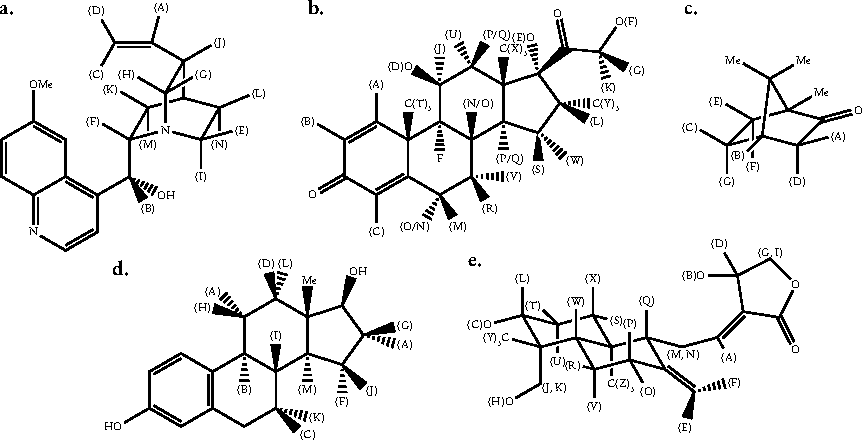
\includegraphics{structures/structures_final.pdf}
    \caption[
        The molecular structures of species giving rise to the experimental
        \acs{NMR} datasets considered in this work.
    ]{
        The molecular structures of species giving rise to the experimental
        \acs{NMR} datasets considered in this work.
        \textbf{a.} Quinine,
        \textbf{b.} Dexamethasone,
        \textbf{c.} Camphor,
        \textbf{d.} 17\textbeta-estradiol,
        \textbf{e.} Andrographolide.
        Proton environments giving rise to signals which are considered in this
        work are denoted with bracketed alphabetical characters. Non-bracketed
        alphabetical characters denote chemical symbols. \ch{Me} denotes the methyl
        group, equivalent to \ch{CH3}.
        \note{
            TODO: check assignments (esp. estradiol). If more structures need
            adding, edit the ChemDraw file on Chive called
            \path{simon_stuff/thesis_structures.cdxml}. Use EB-Garamond for
            atom labels. One a structure is made, scale to 75\% of original
            size, and set font to 7pt. Then in inkscape, rescale this by
            multiplying by 0.8.
            Dexamethasone: replace (J) with (H), (K) with (I), etc...
        }
    }
    \label{fig:structures}
\end{figure}

\subsection{\acs{1D} datasets}
Both the andrographolide and cyclosporin A pulse-acquire experiments were
acquired \textsc{Bruker}'s \texttt{zg30} pulse sequence, which involves
applying a pulse with a target flip angle of \ang{30}, followed by acquisition.
The cyclosporin A pulse-acquire dataset was taken from \textsc{Bruker}'s
\textsc{Topspin} software (v 4.0.8), located at
\path{<TOPSPINROOT>/topspin4.0.8/examdata/exam1d_1H/1}.


\begin{table}[h!]
\centering
\begin{tabular}{ccc}
\hline
 & Andrographolide & Cyclosporin A\\
\hline
$f_{\text{bf}}$ (\unit{\mega\hertz}) & 600.18 & 500.13\\
$\foff$ (\unit{\hertz}) & 2400.7 & 2249.2\\
$\foff$ (\unit{\partspermillion}) & 4 & 4.4972\\
$\fsw$ (\unit{\hertz}) & 4795.4 & 5494.5\\
$\fsw$ (\unit{\partspermillion}) & 7.9899 & 10.986\\
$N$ & 16384 & 65384\\
NS & 1 & 16\\
DS & 0 & 2\\
PLW1 (\unit{\watt}) & 24 & ?\\
P1 (\unit{\micro\second}) & 12 & 10.8\\
D1 (\unit{\second}) & 1 & 1\\

\hline
\end{tabular}
\caption[
    Noteworthy experiment parameters for the pulse-acquire datasets used.
]{
    Noteworthy experiment parameters for the pulse-acquire datasets used.
    NS: Number of scans,
    DS: Number of dummy scans,
    PLW1: Hard pulse power (\unit{\watt}),
    P1: Duration of $\nicefrac{\pi}{2}$ pulse,
    D1: Duration of relaxation delay.
    N.B. The duration of the pulse used was \nicefrac{1}{3} that of P1.
    PLW1 for the cyclosporin dataset could not be found.
}
\label{tab:onedim-params}
\end{table}


\subsection{Diffusion datasets}
The andrographolide diffusion dataset (\cref{fig:andrographolide-dosy})
was acquired using the one-shot \ac{DOSY} pulse sequence\cite{Pelta2002}
(version 1.0c, published on \formatdate{27}{03}{2012}), accessible via the webpage
\url{https://www.nmr.chemistry.manchester.ac.uk/?q=node/264}. The pulse
sequence is displayed in \cref{fig:oneshot-dosy}.


\null\vfill
\begin{table}[h!]
\centering
\begin{tabular}{ccc}
\hline
 & Andrographolide & Glucose/valine/threonine\\
\hline
$f_{\text{bf}}$ (\unit{\mega\hertz}) & 600.18 & 499.98\\
$\foff$ (\unit{\hertz}) & 3000.9 & 2499.9\\
$\foff$ (\unit{\partspermillion}) & 5 & 5\\
$\fsw$ (\unit{\hertz}) & 7211.5 & 10000\\
$\fsw$ (\unit{\partspermillion}) & 12.016 & 20.001\\
$N$ & 16384 & 65536\\
NS & 4 & 32\\
DS & 2 & 4\\
PLW1 (\unit{\watt}) & 24 & 18.204\\
P1 (\unit{\micro\second}) & 12 & 10\\
D1 (\unit{\second}) & 1.5 & 6\\

\hline
\end{tabular}
\caption[
    Noteworthy experiment parameters for the diffusion datasets used.
]{
    Noteworthy experiment parameters for the diffusion datasets used.
    NS: Number of scans,
    DS: Number of dummy scans,
    PLW1: Hard pulse power (\unit{\watt}),
    P1: Duration of $\nicefrac{\pi}{2}$ pulse,
    D1: Duration of relaxation delay.
}
\label{tab:onedim_params}
\end{table}
\vfill\null


The glucose/valine/threonine diffusion dataset (\cref{fig:gluc_val_thre})
was acquired using Bruker's \texttt{ledbpgp2s} pulse sequence (version 1.9, published on
\formatdate{19}{02}{2011}). This is a stimulated echo pulse sequence, featuring
bipolar gradients and a \ac{LED} component\cite{Wu1995}. The pulse sequence is
displayed in \cref{fig:ledbpgp2s}.
Analysis of the dataset using the multivariate methods \ac{DECRA} and
\ac{SCORE} was facilitated through use of The University of Manchester's
\ac{GNAT} software\cite{Castanar2018}.

\begin{figure}[H]
    \centering
    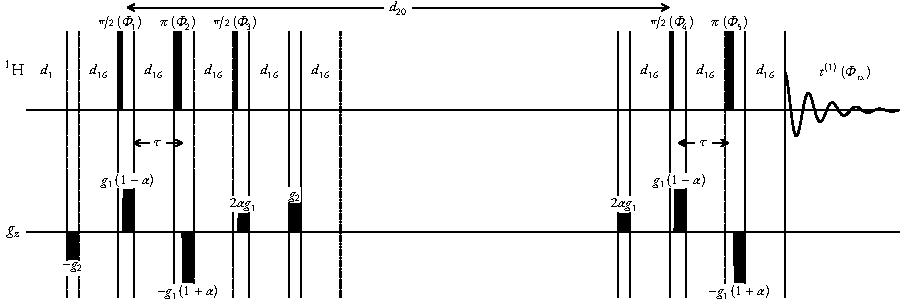
\includegraphics{oneshot_dosy_pulse_sequence/oneshot_dosy_pulse_sequence.pdf}
    \caption[
        Oneshot \acs{DOSY} pulse sequence used for the acquisition of
        andrographolide data.
    ]{
        Oneshot \ac{DOSY} pulse sequence used for the acquisition of
        andrographolide data (\cref{fig:andrographolide-dosy}). All
        delays are included, though they are not to scale.
        Delays:
        $d_1$ (relaxation delay): \qty{1.5}{\second},
        $d_{16}$ (gradient recovery delay): \qty{200}{\micro\second},
        $d_{20}$ (diffusion time, equivalent to $\Delta$): \qty{0.1}{\second}.
        Hard pulses had a power of \qty{24}{\watt},
        with the duration of the $\nicefrac{\pi}{2}$ pulse being
        \qty{12}{\micro\second}.
        Diffusion encoding gradients had a smoothed square profile
        (\texttt{SMSQ10.100}), a duration of \qty{1}{\milli\second}, and had
        strengths related to the values $g_1$ and $\alpha = 0.2$.
        $g_1$ was varied across increments, with the values used
        being (\unit{\gauss \per \centi \meter}):
        6.270,
        12.470,
        16.483,
        19.695,
        22.451,
        24.905,
        27.137,
        29.200,
        31.126,
        32.939,
        34.658,
        36.296,
        37.862,
        39.367,
        40.816,
        42.215,
        43.570,
        44.883,
        46.159,
        47.401.
        Spoiler gradients had the same \texttt{SMSQ10.100} profile, had a
        duration of \qty{600}{\micro\second}, and a strength which was 75\% of
        $g_1$.
        The phase cycling scheme used was:
        $\Phi_1: 2 \times (\ang{0}, \ang{180})$;
        $\Phi_2: 4 \times \ang{0}$;
        $\Phi_3: 4 \times \ang{0}$;
        $\Phi_4: 2 \times \ang{0}, 2 \times \ang{180}$;
        $\Phi_5: 4 \times \ang{0}$;
        $\Phi_{\text{rx}}: \ang{0}, \ang{180}, \ang{180}, \ang{0}$.
    }
    \label{fig:oneshot-dosy}
\end{figure}

\begin{figure}[H]
    \centering
    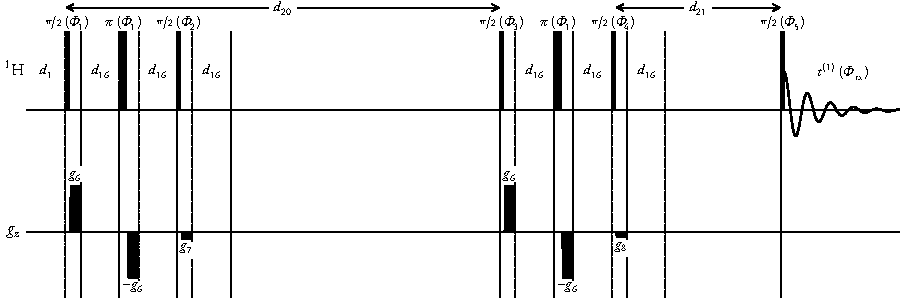
\includegraphics{ledbpgp_pulse_sequence/ledbpgp_pulse_sequence.pdf}
    \caption[
        Pulse sequence used for the acquisition of glucose/threonine/valine
        diffusion data.
    ]{
        Pulse sequence used for the acquisition of glucose/threonine/valine
        diffusion data (\cref{fig:gluc_val_thre}). All
        delays are included, though they are not to scale.
        Delays:
        $d_1$ (relaxation delay): \qty{6}{\second},
        $d_{16}$ (gradient recovery delay): \qty{200}{\micro\second},
        $d_{20}$ (diffusion time, equivalent to $\Delta$): \qty{0.1}{\second},
        $d_{21}$ (eddy-current delay): \qty{5}{\milli\second}.
        Hard pulses had a power of \qty{18.204}{\watt},
        with the duration of the $\nicefrac{\pi}{2}$ pulse being
        \qty{10}{\micro\second}.
        All gradients had a smoothed square profile
        (\texttt{SMSQ10.100}).
        Gradients for diffusion encoding had a duration of
        \qty{1}{\milli\second}, with strength $g_6$ varied across increments,
        with the values used being (\unit{\gauss \per \centi \meter}):
        4.500,
        12.728,
        17.428,
        21.107,
        24.233,
        27.000,
        29.508,
        31.820,
        33.974,
        36.000.
        Spoiler gradients had a duration of \qty{600}{\micro\second}. The
        gradients had the relative strengths $g_7=-0.1713g_6$ and
        $g_8=-0.1317g_6$.
        The phase cycling scheme used was:
        $\Phi_1: 32 \times \ang{0}$;
        $\Phi_2: 8 \times (2 \times \ang{0}, 2 \times \ang{180})$;
        $\Phi_3: 2 \times (4 \times \ang{0}, 4 \times \ang{180}, 4 \times \ang{90}, 4 \times \ang{270})$;
        $\Phi_4: 2 \times (2 \times (\ang{0}, \ang{180}), 2 \times (\ang{180}, \ang{0}), 2 \times (\ang{90}, \ang{270}), 2 \times (\ang{270}, \ang{90})$;
        $\Phi_5: 2 \times (4 \times \ang{0}, 4 \times \ang{180}, 4 \times \ang{90}, 4 \times \ang{270})$;
        $\Phi_{\text{rx}}: 2 \times (\ang{0}, \ang{180}, \ang{180}, \ang{0}, \ang{180}, \ang{0} \ang{0}, \ang{180},
        \ang{270}, \ang{90}, \ang{90}, \ang{270}, \ang{90}, \ang{270}, \ang{270}, \ang{90})$.
    }
    \label{fig:ledbpgp2s}
\end{figure}


\subsection{\acs{2DJ} datasets}
\label{subsec:cupid-experimental}

The 2D J-Resolved datasets presented were acquired using Bruker's
\texttt{jresqf} pulse sequence (version 1.7, released
\formatdate{31}{01}{2012}). This pulse sequence comprises
 $\nicefrac{\pi}{2}(\Phi_1) \rightarrow \nicefrac{\tone}{2} \rightarrow
\pi(\Phi_{2}) \rightarrow \nicefrac{\tone}{2} \rightarrow \ttwo(\Phi_{\text{rx}})$, with
the EXORCYCLE phase-cycling scheme\cite[Section 11.6]{Keeler2010}:
\begin{equation*}
    \begin{array}{lllll}
        \Phi_{1}: & \ang{0} & \ang{0} & \ang{0} & \ang{0} \\
        \Phi_{2}: & \ang{0} & \ang{90} & \ang{180} & \ang{270} \\
        \Phi_{\text{rx}}: & \ang{0} & \ang{180} & \ang{0} & \ang{180}
    \end{array}
\end{equation*}
Key experiment parameters are provided in \cref{tab:jres_params}.

\null\vfill
\begin{table}[h!]
\centering
\begin{tabular}{ccccc}
\hline
 & Quinine & Dexamethasone & Camphor & Estradiol\\
\hline
$f_{\text{bf}}$ (\unit{\mega\hertz}) & 500.13 & 600.18 & 500.13 & 500.3\\
$\fofftwo$ (\unit{\hertz}) & 2500 & 2815.4 & 1000 & 2501.5\\
$\fswone$ (\unit{\hertz}) & 50 & 50 & 50 & 100\\
$\fswtwo$ (\unit{\hertz}) & 7500 & 7211.5 & 5000 & 5000\\
$\fswtwo$ (\unit{\partspermillion}) & 14.996 & 12.016 & 9.9974 & 9.994\\
$\None$ & 128 & 64 & 128 & 128\\
$\Ntwo$ & 16384 & 8192 & 16384 & 16384\\
NS & 4 & 2 & 4 & 4\\
DS & 4 & 8 & 4 & 2\\
PLW1 (\unit{\watt}) & 20.893 & 24 & 20.893 & 31.537\\
P1 (\unit{\micro\second}) & 10 & 12 & 10 & 15\\
D1 (\unit{\second}) & 2 & 1.5 & 2 & 1\\

\hline
\end{tabular}
\caption[
    Noteworthy experiment parameters for the 2D J-Reolved and PSYCHE experiments used.
]{
    Noteworthy experiment parameters for the 2D J-Reolved and PSYCHE experiments used.
    NS: Number of scans,
    DS: Number of dummy scans,
    PLW1: Hard pulse power (\unit{\watt}),
    P1: Duration of $\nicefrac{\pi}{2}$ pulse,
    D1: Duration of relaxation delay.
}
\label{tab:jres_params}
\end{table}
\vfill\null


\subsection{\acs{PSYCHE} datasets}
The pulse sequence used for the acquisition of the estradiol \ac{PSYCHE}
spectrum (\cref{fig:estradiol-cupid}) is presented in
\cref{fig:psyche}, where
pulses, gradients, and delays are described in detail. Equivalent parameters
were used for the basic setup as the estradiol 2DJ experiment, given in
\cref{tab:jres_params}.

The pure shift spectrum of dexamethasone (\cref{fig:dexamethasone-cupid}.a) was
acquired using a \ac{TSE-PSYCHE}
experiment (\cref{fig:tse_psyche}). The pulse sequence file
\texttt{UoM\_1d\_if\_tsepsyche\_ts4x} can be obtained via the link
\url{https://research.manchester.ac.uk/en/datasets/manchester-pure-shift-nmr-workshop-bruker-software}.

\begin{figure}[H]
    \centering
    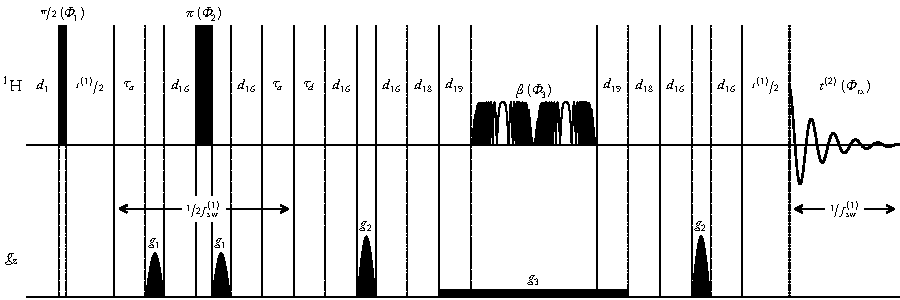
\includegraphics{psyche_pulse_sequence/psyche_pulse_sequence.pdf}
    \caption[
        \acs{PSYCHE} pulse sequence used for the acquisition of estradiol data.
    ]{
        \acs{PSYCHE} pulse sequence used for the acquisition of estradiol data. All
        delays are included, though they are not to scale.
        Delays:
        $d_1$ (relaxation delay): \qty{1}{\second},
        $d_{16}$: (gradient recovery delay): \qty{200}{\micro\second},
        $d_{18}$: \qty{200}{\micro\second},
        $d_{19}$: \qty{1}{\milli\second},
        $\tau_a$: \qty{1.3}{\milli\second},
        $\tau_d$: \qty{18.9}{\milli\second}.
        The \ac{PSYCHE} element featured two saltire chirp pulses with a
        \ac{WURST}\cite{ODell2013}
        amplitude envelope, with a target flip angle $\beta = \ang{20}$.
        Each saltire pulse
        had a bandwidth of \qty{10}{\kilo\hertz},
        a duration of \qty{25}{\milli\second},
        and a power of \qty{280}{\micro\watt}.
        Hard pulses
        had a power of \qty{31.537}{\watt},
        with the duration of the $\nicefrac{\pi}{2}$ pulse being \qty{15}{\micro\second}.
        $G_1$ and $G_2$ were gradients for coherence order selection.
        Each comprised a 100-point sine shape profile, and lasted
        \qty{1}{\milli\second}.
        $G_3$ was a rectangular weak gradient applied during the PSYCHE
        element, with a duration of \qty{52}{\milli\second}.
        The gradeint strengths as a percentage of the maximum permissible
        z-gradient were, respectively 31\%, 47\%, 1.6\%.
        The phase cycling scheme used was:
        $\Phi_1: 2 \times (\ang{0}, \ang{180})$;
        $\Phi_2: 4 \times \ang{0}$;
        $\Phi_3: 2 \times \ang{0}, 2 \times \ang{90}$;
        $\Phi_{\text{rx}}: \ang{0}, \ang{180}, \ang{180}, \ang{0}$.
    }
    \label{fig:psyche}
\end{figure}

\begin{figure}[H]
    \centering
    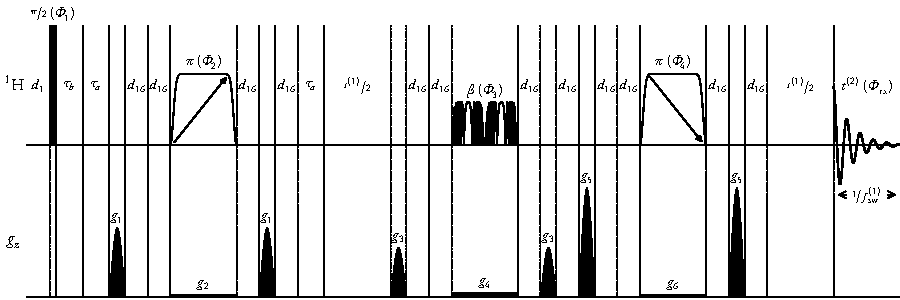
\includegraphics{tse_psyche_pulse_sequence/tse_psyche_pulse_sequence.pdf}
    \caption[
    \acs{TSE-PSYCHE} pulse sequence used for the acquisition of dexamethasone data.
    ]{
        \acs{TSE-PSYCHE} pulse sequence used for the acquisition of dexamethasone
        data (\cref{fig:dexamethasone-cupid}.a).
        Delays:
        $d_1$ (relaxation delay): \qty{2}{\second},
        $d_{16}$: (gradient recovery delay): \qty{200}{\micro\second},
        $\tau_a$: \qty{5}{\milli\second} ($= \nicefrac{1}{4
        f_{\text{sw}}^{(1)}}$).
        The hard $\nicefrac{\pi}{2}$ pulse had a duration of
        \qty{12}{\micro\second}, and a power of \qty{24}{\watt}.
        The two $\pi$ pulses were unidirectional frequency-swept (chirped) pulses,
        with the first pulse sweeping from low to high frequencies, and the second
        pulse sweeping from high to low. These each had a \acs{WURST} amplitude
        envelope, lasted a duration of \qty{40}{\milli\second}, and had a power
        of $\qty{11.05}{\milli\watt}$.
        The \ac{PSYCHE} element had a target flip angle $\beta = \ang{15}$, and
        featured two saltire chirp pulses. Both saltire pulses had a
        \ac{WURST} amplitude envelope, a duration of \qty{15}{\milli\second},
        and a power of
        \qty{1.28}{\milli\watt}.
        $g_1$, $g_3$ and $g_5$ were gradients for coherence order selection.
        Each comprised a 100-point sine profile, and lasted
        \qty{1}{\milli\second}. $g_2$, $g_4$ and $g_6$ were weak rectangular gradients
        which were applied at the same time as the chirped pulses.
        The magnitudes of gradients $g_1$ to  $g_6$ as a percentage of the
        maximum permitted gradient were, respectively:
        49\%, 2\%, 35\%, 3\%, 77\%, 2\%.
        The phase cycling scheme used was:
        $\Phi_1: 8 \times \ang{0}$;
        $\Phi_2: 2 \times (2 \times \ang{0}, 2 \times \ang{180})$;
        $\Phi_3: 2 \times (\ang{0}, \ang{90}), 2 \times (\ang{180}, \ang{270})$;
        $\Phi_4: 8 \times \ang{0}$;
        $\Phi_{\text{rx}}: 4 \times (\ang{0}, \ang{180})$.
    }
    \label{fig:tse_psyche}
\end{figure}

\section{\acs{CUPID} result metrics}
\note{Needs updating: replace sucrose with strychnine, re-order according to the order in the thesis}.
\begin{landscape}
    \begin{longtable}{cccccccc}
        \caption[
            Metrics for all the results generated using \acs{CUPID}.
        ]
        {
            Metrics for all the results generated using \acs{CUPID}
            (\cref{subsec:cupid-results}) The \emph{Initial} $M$ specifies
            the number of oscillators given to the MMEMP. Values with a *
            indicate that they were
            determined by applying the MDL on the first direct-dimension slice
            of the data. Values with a \textsuperscript{\textdagger} indicate
            that they were manually provided. The \emph{M after MMEMP} column
            indicates how many oscillators were present in the initial guess
            $\symbf{\theta}^{(0)}$. This can differ from \emph{Initial M}, as
            any oscillators possessing negative damping factors in the MMEMP
            result were purged. The \emph{M after NLP} column indicates
            how many oscillators were present in $\symbf{\theta}^{(*)}$, the
            result of non-linear programming. When this value
            is smaller than \emph{M after MMEMP}, negative-amplitude
            oscillators were found and purged during the optimisation.
            \emph{Purged oscillators} indicates how many oscillators were
            removed from the final estimation result, based on the first-order
            signal criteria outlined in \cref{subsec:mp-selection}.
        }
        \label{tab:cupid-metrics}\\
        \hline
        Region (\unit{\partspermillion}) &
        Initial $M$ &
        MMEMP time  (\unit{\second}) &
        $M$ after MMEMP &
        NLP time (\unit{\second}) &
        NLP iterations &
        $M$ after NLP &
        Purged oscillators \\
        \hline
        \endfirsthead
        \hline
        Region (\unit{\partspermillion}) &
        Initial $M$ &
        MMEMP time  (\unit{\second}) &
        $M$ after MMEMP &
        NLP time (\unit{\second}) &
        NLP iterations &
        $M$ after NLP &
        Purged oscillators \\
        \hline
        \endhead
        \hline
        \endlastfoot
        \hline
        \multicolumn{8}{r}{Continues on next page...}\\
        \hline
        \endfoot
        \multicolumn{8}{c}{\textbf{Quinine}}\\
        \hline
        5.8 -- 5.55 &
        18* &
        11.2 &
        18 &
        61.4 &
        124 &
        10 &
        None\\
        5 -- 4.85 &
        17\textsuperscript{\textdagger} &
        3.5 &
        17 &
        32.1 &
        47 &
        17 &
        None\\
        3.75 -- 3.63 &
        15* &
        2.4 &
        15 &
        34.7 &
        69 &
        13 &
        None\\
        3.17 -- 3.06 &
        15* &
        1.9 &
        15 &
        67.9 &
        150 &
        10 &
        None\\
        2.8 -- 2.6 &
        25\textsuperscript{\textdagger} &
        7.5 &
        25 &
        112.9 &
        125 &
        22 &
        None\\
        2 -- 1.7 &
        40\textsuperscript{\textdagger} &
        19.8 &
        40 &
        233.3 &
        150 &
        37 &
        1\\
        1.64 -- 1.52 &
        20* &
        2.8 &
        20 &
        38.4 &
        55 &
        18 &
        None\\
        1.52 -- 1.4 &
        14* &
        2.6 &
        13 &
        26.6 &
        58 &
        12 &
        None\\
        \hline
        \multicolumn{8}{c}{\textbf{Estradiol}}\\
        \hline
        2.29 -- 2.17 &
        20\textsuperscript{\textdagger} &
        11.5 &
        17 &
        31.7 &
        150 &
        11 &
        2\\
        2.12 -- 2 &
        15\textsuperscript{\textdagger} &
        11.4 &
        15 &
        27.9 &
        150 &
        9 &
        3\\
        1.95 -- 1.72 &
        40\textsuperscript{\textdagger} &
        42.7 &
        40 &
        93.2 &
        125 &
        34 &
        4\\
        1.65 -- 1.52 &
        20\textsuperscript{\textdagger} &
        12.2 &
        19 &
        47.9 &
        150 &
        15 &
        2\\
        1.45 -- 1.02 &
        90\textsuperscript{\textdagger} &
        65.6 &
        86 &
        271.3 &
        150 &
        80 &
        8\\
\hline
\multicolumn{8}{c}{\textbf{Sucrose}}\\
\hline
6.08 -- 5.91 &
2* &
0.7 &
2 &
0.3 &
10 &
2 &
None\\
4.72 -- 4.46 &
16\textsuperscript{\textdagger} &
2.2 &
16 &
3.5 &
21 &
16 &
None\\
4.46 -- 4.22 &
16\textsuperscript{\textdagger} &
2.1 &
16 &
4.5 &
32 &
16 &
None\\
4.22 -- 4.1 &
4\textsuperscript{\textdagger} &
0.5 &
4 &
3.2 &
95 &
4 &
None\\
4.09 -- 3.98 &
6* &
0.3 &
6 &
0.9 &
12 &
6 &
None\\
3.98 -- 3.83 &
10\textsuperscript{\textdagger} &
0.6 &
10 &
2.9 &
31 &
10 &
None\\
3.58 -- 3.28 &
12* &
2.5 &
12 &
3.0 &
26 &
12 &
None\\
2.08 -- 1.16 &
3* &
3.9 &
3 &
0.4 &
9 &
3 &
None\\
1.05 -- 0.0 &
8* &
4.0 &
8 &
1.1 &
10 &
8 &
None\\
\hline
\multicolumn{8}{c}{\textbf{Four Multiplets (Run 1)}}\\
\hline
0.06 -- -0.06 &
34\textsuperscript{\textdagger} &
3.2 &
34 &
45.7 &
65 &
33 &
1\\
\hline
\multicolumn{8}{c}{\textbf{Four Multiplets (Run 2)}}\\
\hline
0.06 -- -0.06 &
38\textsuperscript{\textdagger} &
4.2 &
38 &
76.9 &
105 &
32 &
None\\
\hline
\multicolumn{8}{c}{\textbf{Four Multiplets (Run 3)}}\\
\hline
0.06 -- -0.06 &
39\textsuperscript{\textdagger} &
4.3 &
38 &
27.6 &
35 &
32 &
None\\
\hline
\multicolumn{8}{c}{\textbf{Four Multiplets (Run 4)}}\\
\hline
0.06 -- -0.06 &
40\textsuperscript{\textdagger} &
4.2 &
40 &
45.6 &
61 &
32 &
None\\
\hline
\multicolumn{8}{c}{\textbf{Four Multiplets (Run 5)}}\\
\hline
0.06 -- -0.06 &
37\textsuperscript{\textdagger} &
3.5 &
37 &
74.8 &
100 &
33 &
1\\
\hline
\multicolumn{8}{c}{\textbf{Camphor}}\\
\hline
2.55 -- 2.475 &
9* &
2.0 &
8 &
40.6 &
150 &
6 &
1 \\
2.35 -- 2.23 &
18* &
5.7 &
18 &
68.3 &
100 &
18 &
None\\
2.09 -- 2.025 &
8* &
1.3 &
18 &
18.3 &
96 &
3 &
None\\
1.95 -- 1.75 &
35* &
19.9 &
32 &
260.2 &
225 &
30 &
None\\
1.7 -- 1.61 &
21* &
3.9 &
21 &
72.3 &
84 &
21 &
1 \\
1.375 -- 1.215 &
29* &
10.6 &
29 &
117.2 &
123 &
22 &
None\\
\hline
\multicolumn{8}{c}{\textbf{Dexamethasone}}\\
\hline
7.45 -- 7.15 &
2\textsuperscript{\dagger} &
0.8 &
2 &
0.5 &
13 &
2 &
None\\
6.4 -- 5.9 &
15* &
4.4 &
7 &
14.2 &
66 &
7 &
None\\
5.5 -- 4.8 &
3\textsuperscript{\dagger} &
4.0 &
3 &
1.1 &
17 &
3 &
None\\
4.8 -- 4.3 &
11* &
3.2 &
11 &
12.7 &
58 &
9 &
2 \\
4.25 -- 3.97 &
20\textsuperscript{\dagger} &
1.1 &
19 &
35.2 &
133 &
17 &
0 \\
3 -- 2.87 &
13* &
0.3 &
11 &
48.8 &
219 &
10 &
None \\
2.68 -- 2.43 &
23* &
1.2 &
18 &
68.2 &
250 &
14 &
None \\
2.413 -- 2.26 &
18* &
0.395 &
17 &
61.7 &
197 &
15 &
None \\
2.195 -- 2.034 &
17* &
0.4 &
17 &
61.7 &
200 &
17 &
None \\
1.85 -- 1.7 &
12* &
0.4 &
10 &
15.0 &
79 &
9 &
None\\
1.7 -- 1.25 &
30* &
3.2 &
30 &
127.2 &
250 &
27 &
8 \\
1.14 -- 1 &
12* &
0.4 &
10 &
36.9 &
183 &
10 &
3 \\
1 -- 0.65 &
3\textsuperscript{\textdagger} &
2.0 &
3 &
0.9 &
17 &
3 &
None\\
\end{longtable}
\end{landscape}
